% !TEX root = manuscript.tex
\documentclass[12pt]{article}

\usepackage[margin=1in]{geometry}
\usepackage{fontspec}
\IfFontExistsTF{Times New Roman}{\setmainfont{Times New Roman}}{\setmainfont{TeX Gyre Termes}}
\usepackage{booktabs}
\usepackage{array}
\usepackage{tabularx}
\usepackage{float}
\usepackage{caption}
\usepackage{setspace}
\usepackage{enumitem}
\usepackage{xcolor}
\usepackage{eso-pic}
\usepackage{siunitx}
\usepackage{pgfplots}
\usepackage{pgfplotstable}
\usepgfplotslibrary{groupplots}
\usepackage[hidelinks]{hyperref}

\setstretch{1.0}
\setcounter{secnumdepth}{0}
\captionsetup{font=small, labelfont=bf}
\sisetup{round-mode=places, round-precision=4}
\pgfplotsset{compat=1.18}
\pgfplotstableset{col sep=comma}
\makeatletter
\renewcommand{\@biblabel}[1]{#1.}
\makeatother

\newcommand{\DataDir}{../outputs/latex_data}
\definecolor{LogRegColor}{HTML}{E74C3C}
\definecolor{RFColor}{HTML}{2980B9}
\definecolor{HGBColor}{HTML}{27AE60}
\definecolor{MLPColor}{HTML}{8E44AD}
\definecolor{EnsColor}{HTML}{D35400}
\definecolor{UCIRed}{HTML}{C0392B}
\definecolor{NHBlue}{HTML}{2471A3}
\definecolor{TWGreen}{HTML}{1E8449}

\pgfplotsset{
  ckdaxis/.style={
    width=\linewidth,
    height=0.48\linewidth,
    grid=major,
    grid style={draw=gray!20},
    tick align=inside,
    tick pos=left,
    tick style={black},
    tick label style={font=\small},
    label style={font=\small},
    title style={font=\bfseries\small},
    legend style={font=\scriptsize, draw=none, fill=none, cells={anchor=west}},
    unbounded coords=jump
  }
}

\newcommand{\PlotFiveModelCurves}[1]{
  \addplot+[mark=o, thick, color=LogRegColor] table[x=train_size,y=LogReg_test] {#1};
  \addlegendentry{Logistic}
  \addplot+[mark=square*, thick, color=RFColor] table[x=train_size,y=RF_test] {#1};
  \addlegendentry{Random forest}
  \addplot+[mark=triangle*, thick, color=HGBColor] table[x=train_size,y=HGB_test] {#1};
  \addlegendentry{Gradient boosting}
  \addplot+[mark=diamond*, thick, color=MLPColor] table[x=train_size,y=MLP_test] {#1};
  \addlegendentry{MLP}
  \addplot+[mark=*, thick, color=EnsColor] table[x=train_size,y=Ensemble_test] {#1};
  \addlegendentry{Ensemble}
}

\newcommand{\PlotFiveModelCurvesNoLegend}[1]{
  \addplot+[mark=o, thick, color=LogRegColor, forget plot] table[x=train_size,y=LogReg_test] {#1};
  \addplot+[mark=square*, thick, color=RFColor, forget plot] table[x=train_size,y=RF_test] {#1};
  \addplot+[mark=triangle*, thick, color=HGBColor, forget plot] table[x=train_size,y=HGB_test] {#1};
  \addplot+[mark=diamond*, thick, color=MLPColor, forget plot] table[x=train_size,y=MLP_test] {#1};
  \addplot+[mark=*, thick, color=EnsColor, forget plot] table[x=train_size,y=Ensemble_test] {#1};
}

\title{\textbf{When Perfect Is Wrong: Exposing the AUC $\approx$ 1.0 Illusion in Chronic Kidney Disease Machine Learning Benchmarks}}
\author{Justin Xia\\American Heritage School, Plantation, FL}
\date{}

\begin{document}
\color{black}
\AddToShipoutPictureBG{\AtPageLowerLeft{\color{white}\rule{\paperwidth}{\paperheight}}}
\maketitle

\begin{abstract} 
Chronic kidney disease (CKD) affects about 9--10\% of the global population, yet many machine-learning studies for early detection still rely on the UCI CKD dataset ($n=400$) and report area-under-the-curve (AUC) values near 1.0. This study asks whether those results reflect algorithmic progress or a benchmark ceiling effect. We analyze three public CKD datasets as separate prediction tasks: UCI CKD, NHANES 2021--2023, and the Tawam Hospital UAE cohort. Five models are compared using stratified train/test splits, repeated learning curves, single-feature screening, NHANES feature-set sensitivity analysis, UCI feature ablation, calibration checks, Tawam train/test gap analysis, and UCI-to-external cross-dataset transfer. The revised pipeline uses train-only preprocessing, one-hot encoding for UCI nominal variables, explicit ordered encoding for clinically ordered UCI variables, and 20 repeated subsamples per learning-curve point. UCI remains effectively saturated, with all models near AUC 1.0. NHANES shows label-feature circularity: removing eGFR/ACR and then creatinine/BUN surrogates substantially lowers performance. Tawam yields lower and more realistic AUC values and continues improving with additional training data. UCI-trained models transfer weakly and inconsistently to NHANES and Tawam using shared clinical features. These results suggest that UCI is useful for teaching and code validation, but not as a general benchmark for advancing CKD machine learning or as standalone evidence of clinical utility.
\end{abstract}

\noindent\textbf{Keywords:} chronic kidney disease, machine learning, AUC, benchmark validity, learning curves, clinical informatics, shortcut learning, external validation

\section{Introduction}
\subsection{Background and Context}
Chronic kidney disease is a common progressive condition that affects about 9--10\% of the global population and is often diagnosed after substantial renal decline has already occurred \cite{bikbov2020,levey2012}. This clinical gap has motivated extensive work on CKD recognition, risk prediction, and prognosis using routine laboratory and demographic data \cite{islam2023,chittora2021,dritsas2022,halder2024,chen2025,li2025,shu2026}. In the published machine-learning literature, however, one benchmark dominates: the UCI CKD dataset \cite{rubini2015}. Studies using UCI often report near-perfect discrimination across many model families \cite{salekin2016,chittora2021,ganie2023}, which creates a basic scientific question: when common models reach AUC $\approx 1.0$, are we measuring model quality or benchmark triviality?

\subsection{Benchmark Validity}
A useful benchmark should be hard enough to distinguish methods and aligned enough with the intended clinical task that good benchmark performance has external meaning. Clinical prediction reporting guidelines emphasize transparent outcome definitions, validation, calibration, and the limits of model transportability \cite{collins2024}. Medical-AI studies also show that strong internal performance can fail under external validation when models learn site-specific or shortcut signals \cite{zech2018,geirhos2020,ongly2024,hill2024}. UCI represents a prevalent-disease hospital recognition task. NHANES represents a cross-sectional epidemiological classification task, where the CKD label is partly defined by variables that may also appear as predictors. Tawam represents incident CKD progression over long follow-up in a high-cardiovascular-risk cohort \cite{alshamsi2018}. These are not exchangeable prediction problems, so this paper treats them as task-specific case studies rather than as a single leaderboard.

\subsection{Study Objectives}
This study evaluates whether the near-perfect performance often reported on UCI is a property of strong algorithms or of an unusually easy benchmark. The revised analysis addresses reviewer concerns by adding UCI-to-external transfer, three NHANES feature sets, stratified repeated learning curves, corrected UCI categorical preprocessing, UCI ablation, Tawam overfitting checks, calibration and threshold summaries, and a KDIGO stage mapping.

\section{Methods}
\subsection{Datasets}
\begin{table}[H]
\centering
\caption{Summary of datasets used in this study \cite{rubini2015,cdc2024,alshamsi2018}.}
\small
\renewcommand{\arraystretch}{1.18}
\setlength{\tabcolsep}{5pt}
\begin{tabularx}{\textwidth}{|>{\raggedright\arraybackslash}p{2.2cm}|>{\centering\arraybackslash}p{1.1cm}|>{\raggedright\arraybackslash}X|>{\raggedright\arraybackslash}X|>{\raggedright\arraybackslash}X|}
\hline
\textbf{Dataset} & \textbf{N} & \textbf{Origin} & \textbf{CKD label} & \textbf{Key features} \\
\hline
UCI CKD & 400 & India hospital EHR & Physician diagnosis, prevalent CKD & Hemoglobin, specific gravity, creatinine, packed cell volume, albumin \\
\hline
NHANES 2021--2023 & 11,933 & U.S. national health survey & eGFR $<60$ or ACR $\ge 30$ & Creatinine, BUN, albumin, BMI, eGFR, ACR, diabetes, blood pressure \\
\hline
Tawam Hospital UAE & 491 & Abu Dhabi EHR & 8-year CKD progression & Creatinine, eGFR, HbA1c, cholesterol, triglycerides, blood pressure, BMI \\
\hline
\end{tabularx}
\end{table}

\begin{table}[H]
\centering
\caption{Mapping of dataset labels to KDIGO 2024 CKD stages \cite{kdigo2024}.}
\small
\renewcommand{\arraystretch}{1.18}
\setlength{\tabcolsep}{5pt}
\begin{tabularx}{\textwidth}{|>{\raggedright\arraybackslash}p{2.4cm}|>{\raggedright\arraybackslash}X|>{\raggedright\arraybackslash}X|>{\raggedright\arraybackslash}X|}
\hline
\textbf{Dataset} & \textbf{CKD stages represented} & \textbf{Stages excluded} & \textbf{Population setting} \\
\hline
UCI CKD & Primarily G3b--G5 among cases & G1--G3a largely absent & Hospital outpatients/inpatients \\
\hline
NHANES 2021--2023 & G1--G5 by eGFR/ACR criteria & None by definition & U.S. community-dwelling sample \\
\hline
Tawam Hospital UAE & Baseline G1--G2; progression toward $\le$G3b & G4--G5 at baseline excluded & Hospital cardiology cohort \\
\hline
\end{tabularx}
\end{table}

\begin{table}[H]
\centering
\caption{Dataset audit from the regenerated pipeline. Predictor missingness is counted before train-only imputation.}
\small
\renewcommand{\arraystretch}{1.18}
\setlength{\tabcolsep}{6pt}
\resizebox{\textwidth}{!}{%
\begin{tabular}{|l|r|r|r|r|r|r|r|r|r|r|}
\hline
\textbf{Dataset} & \textbf{N} & \textbf{Pos.} & \textbf{Pos. rate} & \textbf{Pred.} & \textbf{Miss.} & \textbf{Train N} & \textbf{Train pos.} & \textbf{Test N} & \textbf{Test pos.} & \textbf{Dup. IDs} \\
\hline
UCI CKD & 400 & 250 & 0.625 & 24 & 1,012 & 300 & 0.627 & 100 & 0.620 & 0 \\
\hline
NHANES 2021--2023 & 11,933 & 8,341 & 0.699 & 11 & 38,655 & 10,143 & 0.699 & 1,790 & 0.699 & 0 \\
\hline
Tawam UAE & 491 & 56 & 0.114 & 10 & 21 & 368 & 0.114 & 123 & 0.114 & 0 \\
\hline
\end{tabular}%
}
\end{table}

NHANES cohort construction used the prepared 2021--2023 file with eGFR, albumin-creatinine ratio, CKD stage, and CKD-present columns already available. The analysis script treats the prepared eGFR column as the source kidney-filtration variable and does not recompute eGFR from creatinine, so the exact estimating equation is inherited from the prepared data file rather than from this modeling script. Participants with nonmissing CKD label status were retained. Predictor missingness was not used as an exclusion criterion; those cells were imputed inside the training pipeline. The final NHANES analytic file contained 11,933 participants, 8,341 CKD-positive labels, 11 predictors, and 38,655 missing predictor cells before imputation. This analysis does not use NHANES survey weights, strata, primary sampling units, or laboratory subsample weights because the goal is algorithmic benchmark behavior rather than U.S. population-prevalence estimation; CDC/NCHS guidance notes that the 2021--2023 cycle used a changed post-pandemic sample design and specific weighting/analytic guidance for population estimates \cite{nhanes2024brief}. Because NHANES does not contain every UCI variable, such as hemoglobin and urine specific gravity, and adds variables not available in UCI, such as BMI and diabetes status, AUC-ROC differences are interpreted as task- and feature-set-specific behavior rather than direct evidence that one population is intrinsically easier or harder.

\subsection{Preprocessing}
All train/test splits are stratified by label. Missing predictors are imputed using statistics fit on the training split only, and scaling is also fit on training data only, because preprocessing that uses pooled train/test information can inflate validation performance in small datasets \cite{vabalas2019}. UCI categorical preprocessing was revised to avoid arbitrary numeric ordering: nominal variables are one-hot encoded, while clinically ordered variables such as specific gravity and urine dipstick values use explicit ordered encodings. NHANES is evaluated under three feature sets: all predictors, no eGFR/ACR, and no eGFR/ACR/creatinine/BUN. Tawam excludes identifiers and time-to-event variables from the predictor matrix, and the audit found no duplicate StudyID values.

\subsection{Ethical Considerations}
This study is a secondary analysis of de-identified public or previously published datasets and involved no direct patient contact. The UCI CKD dataset is distributed through the UCI Machine Learning Repository, NHANES is released by CDC/NCHS under its public-use data procedures, and the Tawam cohort was analyzed from the published dataset accompanying the original study, which reported local ethics approval \cite{rubini2015,cdc2024,alshamsi2018}. Therefore, this manuscript did not require new institutional review board review or informed consent collection by the author.

\subsection{Models and Experiments}
\begin{table}[H]
\centering
\caption{Machine-learning models evaluated in the revised pipeline.}
\small
\renewcommand{\arraystretch}{1.18}
\setlength{\tabcolsep}{5pt}
\begin{tabularx}{\textwidth}{|>{\raggedright\arraybackslash}p{2.8cm}|>{\raggedright\arraybackslash}p{2.5cm}|>{\raggedright\arraybackslash}X|>{\raggedright\arraybackslash}X|}
\hline
\textbf{Model} & \textbf{Family} & \textbf{Key hyperparameters} & \textbf{Role} \\
\hline
Logistic Regression & Linear & $C=1.0$, max\_iter=1000 & Interpretable baseline \\
\hline
Random Forest & Bagging ensemble & 200 trees, depth 8, minimum leaf 5 & Nonlinear baseline \\
\hline
Gradient Boosting & Boosting ensemble & 300 iterations, learning rate 0.05, depth 5 & Primary learning-curve model \\
\hline
Neural Network (MLP) & Deep learning & 128--64--32 hidden units, early stopping & Flexible nonlinear model \\
\hline
Soft-voting Ensemble & HGB + RF + MLP & Soft voting over three base learners & Aggregate benchmark \\
\hline
\end{tabularx}
\end{table}

The main experiments are: full-data model comparison; UCI, NHANES, and Tawam learning curves; NHANES feature-set sensitivity; UCI single-feature screening; UCI top-three feature ablation; Tawam train/test gap analysis; and UCI-trained cross-dataset evaluation using the shared clinical subset of age, systolic blood pressure, and serum creatinine. All primary train/test splits use random seed 42, and repeated subsampling experiments use deterministic seed offsets. Area under the receiver operating characteristic curve (AUC-ROC, abbreviated as AUC in tables) is the primary discrimination metric. Brier score and threshold 0.5 sensitivity/specificity are reported for NHANES and Tawam as calibration and threshold summaries, consistent with clinical prediction guidance that discrimination alone is not sufficient for evaluating clinical models \cite{collins2024}.

\subsection{Power-Law Fits}
NHANES learning curves are fit with a descriptive inverse power-law form, a common way to summarize learning behavior as performance changes with sample size \cite{meek2002,dayimu2024}:
\[
\mathrm{AUC}(n)=c-a n^{-b},
\]
where $c$ is constrained to the interval from the maximum observed AUC, or just below 1.0 when the maximum equals 1.0, to 1.0; $a$ is constrained to $[0,200]$; and $b$ is constrained to $[0,5]$. Starting values are $c=\min(1.0,\max(\mathrm{AUC})+0.01)$, $a=2.0$, and $b=0.5$. The script exports bootstrap intervals and a sensitivity refit that excludes the two smallest training sizes. These fits are descriptive summaries of model behavior, not biological limits.
Parameters were estimated by bounded nonlinear least squares. Table 8 reports bootstrap 95\% confidence intervals from 500 resamples and the ceiling from the sensitivity refit that excludes the two smallest training sizes. Estimates equal to 1.000 for $c$ or 200 for $a$ indicate that the constrained optimizer reached the upper bound, so those values should be read as conservative fit summaries rather than as proof of a true asymptotic limit.

\section{Results}
\subsection{Full-Data Comparison}
\begin{table}[H]
\centering
\caption{Held-out test-set performance for the revised pipeline.}
\begingroup
\small
\renewcommand{\arraystretch}{1.15}
\setlength{\tabcolsep}{5pt}
\begin{tabular}{|l|c|c|c|c|c|}
\hline
Model & UCI AUC & NHANES AUC & Tawam AUC & NHANES Brier & Tawam Brier \\
\hline
LogReg & 1.0000 & 0.9457 & 0.8768 & 0.0835 & 0.0612 \\
RF & 0.9996 & 1.0000 & 0.9083 & 0.0043 & 0.0658 \\
HGB & 1.0000 & 1.0000 & 0.9102 & 0.0001 & 0.0576 \\
MLP & 0.9983 & 0.9971 & 0.9083 & 0.0153 & 0.1397 \\
Ensemble & 1.0000 & 1.0000 & 0.9050 & 0.0033 & 0.0663 \\
\hline
\end{tabular}
\endgroup
\end{table}

\begin{figure}[H]
\centering
\begin{tikzpicture}
\begin{axis}[
  ckdaxis,
  ybar,
  bar width=5pt,
  ymin=0.82,
  ymax=1.02,
  symbolic x coords={LogReg,RF,HGB,MLP,Ensemble},
  xtick=data,
  xticklabel style={rotate=25,anchor=east},
  ylabel={AUC-ROC},
  title={Model performance by dataset},
  legend style={at={(0.5,-0.20)}, anchor=north, legend columns=3, font=\scriptsize, draw=none, fill=none}
]
\addplot+[fill=UCIRed, draw=UCIRed] table[x=model,y=UCI] {\DataDir/fig1_model_comparison_wide.csv};
\addlegendentry{UCI}
\addplot+[fill=NHBlue, draw=NHBlue] table[x=model,y=NHANES] {\DataDir/fig1_model_comparison_wide.csv};
\addlegendentry{NHANES}
\addplot+[fill=TWGreen, draw=TWGreen] table[x=model,y=Tawam] {\DataDir/fig1_model_comparison_wide.csv};
\addlegendentry{Tawam}
\end{axis}
\end{tikzpicture}
\caption{UCI is saturated across model families, NHANES with all features is also near-ceiling because of label-feature overlap, and Tawam remains lower and more discriminating among algorithms. The y-axis is intentionally truncated at 0.82 to make small AUC differences visible.}
\end{figure}

\begin{table}[H]
\centering
\caption{Threshold 0.5 sensitivity and specificity for NHANES and Tawam.}
\begingroup
\small
\renewcommand{\arraystretch}{1.15}
\setlength{\tabcolsep}{8pt}
\begin{tabular}{|l|l|c|c|}
\hline
Model & Dataset & Sensitivity & Specificity \\
\hline
LogReg & NHANES & 0.963 & 0.742 \\
LogReg & Tawam & 0.357 & 1.000 \\
RF & NHANES & 1.000 & 1.000 \\
RF & Tawam & 0.143 & 1.000 \\
HGB & NHANES & 1.000 & 1.000 \\
HGB & Tawam & 0.429 & 0.982 \\
MLP & NHANES & 0.989 & 0.961 \\
MLP & Tawam & 0.786 & 0.917 \\
Ensemble & NHANES & 1.000 & 1.000 \\
Ensemble & Tawam & 0.286 & 1.000 \\
\hline
\end{tabular}
\endgroup
\end{table}

\subsection{Learning Curves}
UCI learning curves plateau rapidly. With the full 20-repeat run, gradient boosting rises from roughly 0.79 at $n=40$ to about 0.99 at $n=50$ and reaches the ceiling by the full training size.

\begin{figure}[H]
\centering
\begin{tikzpicture}
\begin{axis}[
  ckdaxis,
  xlabel={UCI training size},
  ylabel={Test AUC-ROC},
  ymin=0.45,
  ymax=1.02,
  xtick={10,20,40,50,75,100,150,200,300},
  title={UCI learning curves},
  legend style={at={(0.5,-0.21)}, anchor=north, legend columns=5, font=\scriptsize, draw=none, fill=none}
]
\PlotFiveModelCurves{\DataDir/fig2_uci_learning_curves_wide.csv}
\end{axis}
\end{tikzpicture}
\caption{UCI performance reaches near-perfect AUC with small stratified subsamples, supporting the ceiling-effect interpretation.}
\end{figure}

\begin{figure}[H]
\centering
\begin{tikzpicture}
\begin{axis}[
  ckdaxis,
  xmode=log,
  xlabel={NHANES training size},
  ylabel={Test AUC-ROC},
  ymin=0.55,
  ymax=1.02,
  title={NHANES learning curves, all features},
  legend style={at={(0.5,-0.21)}, anchor=north, legend columns=5, font=\scriptsize, draw=none, fill=none}
]
\PlotFiveModelCurves{\DataDir/fig3_nhanes_learning_curves_wide.csv}
\end{axis}
\end{tikzpicture}
\caption{With eGFR and ACR included, NHANES approaches a ceiling because the label definition is partly inside the feature set under KDIGO-style eGFR/albuminuria criteria \cite{kdigo2024}.}
\end{figure}

\subsection{NHANES Feature-Set Sensitivity}
\begin{table}[H]
\centering
\caption{NHANES full-data AUC depends strongly on whether label-defining variables are included.}
\begingroup
\small
\renewcommand{\arraystretch}{1.15}
\setlength{\tabcolsep}{7pt}
\begin{tabular}{|l|c|c|c|}
\hline
Model & All features & No eGFR/ACR & No eGFR/ACR/Cr/BUN \\
\hline
LogReg & 0.9457 & 0.8131 & 0.6926 \\
RF & 1.0000 & 0.9737 & 0.9218 \\
HGB & 1.0000 & 0.9751 & 0.9205 \\
MLP & 0.9971 & 0.9690 & 0.9155 \\
Ensemble & 1.0000 & 0.9749 & 0.9216 \\
\hline
\end{tabular}
\endgroup
\end{table}

\begin{figure}[H]
\centering
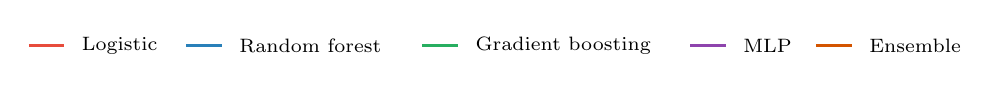
\begin{tikzpicture}
  \draw[thick, color=LogRegColor] (0,0) -- (0.45,0);
  \node[anchor=west, font=\scriptsize] at (0.55,0) {Logistic};
  \draw[thick, color=RFColor] (2.0,0) -- (2.45,0);
  \node[anchor=west, font=\scriptsize] at (2.55,0) {Random forest};
  \draw[thick, color=HGBColor] (5.0,0) -- (5.45,0);
  \node[anchor=west, font=\scriptsize] at (5.55,0) {Gradient boosting};
  \draw[thick, color=MLPColor] (8.4,0) -- (8.85,0);
  \node[anchor=west, font=\scriptsize] at (8.95,0) {MLP};
  \draw[thick, color=EnsColor] (10.0,0) -- (10.45,0);
  \node[anchor=west, font=\scriptsize] at (10.55,0) {Ensemble};
\end{tikzpicture}

\vspace{0.9em}

\begin{tikzpicture}
\begin{groupplot}[
  group style={group size=1 by 3, vertical sep=2.65cm},
  width=0.88\textwidth,
  height=0.22\textwidth,
  grid=major,
  grid style={draw=gray!20},
  xmode=log,
  ymin=0.55,
  ymax=1.02,
  tick align=inside,
  tick pos=left,
  tick label style={font=\small},
  label style={font=\small},
  xlabel style={yshift=-0.25em},
  title style={font=\bfseries\small},
  unbounded coords=jump
]
\nextgroupplot[title={All features}, ylabel={Test AUC}]
\PlotFiveModelCurvesNoLegend{\DataDir/fig9_nhanes_all_wide.csv}
\nextgroupplot[title={No eGFR/ACR}]
\PlotFiveModelCurvesNoLegend{\DataDir/fig9_nhanes_no_egfr_acr_wide.csv}
\nextgroupplot[title={No eGFR/ACR/Cr/BUN}, xlabel={Training size}]
\PlotFiveModelCurvesNoLegend{\DataDir/fig9_nhanes_no_lab_surrogates_wide.csv}
\end{groupplot}
\end{tikzpicture}
\caption{Removing label-defining and closely related laboratory variables exposes a substantially harder NHANES prediction task, especially for logistic regression.}
\end{figure}

\subsection{Tawam Learning Curves and Overfitting}
Tawam is the clearest nontrivial prediction task in this analysis: it does not collapse into either UCI's advanced-disease separation or NHANES's label-feature circularity. The train/test gap remains visible but not catastrophic.

\begin{figure}[H]
\centering
\begin{tikzpicture}
\begin{axis}[
  ckdaxis,
  xlabel={Tawam training size},
  ylabel={AUC-ROC},
  ymin=0.45,
  ymax=1.03,
  xtick={20,30,40,50,75,100,125,150,200,368},
  title={Tawam learning curves with train/test gap},
  legend style={at={(0.5,-0.21)}, anchor=north, legend columns=3, font=\scriptsize, draw=none, fill=none}
]
\PlotFiveModelCurves{\DataDir/fig4_tawam_learning_curves_wide.csv}
\addplot+[mark=none, dashed, thick, color=HGBColor] table[x=train_size,y=HGB_train] {\DataDir/fig4_tawam_learning_curves_wide.csv};
\addlegendentry{HGB train}
\end{axis}
\end{tikzpicture}
\caption{Tawam test AUC improves with additional data. The dashed gradient-boosting training curve shows the monitored overfitting gap.}
\end{figure}

\subsection{Single-Feature Screening and Ablation}
Single-feature screening with logistic regression identifies hemoglobin, serum creatinine, packed cell volume, and specific gravity as highly discriminative individual UCI predictors. Creatinine-based kidney function and albuminuria are central to CKD definition and staging, and anemia-related measures such as hemoglobin are clinically associated with established CKD \cite{levey2012,kdigo2024}. The issue is not that these are invalid variables; the issue is that they make this hospital case-control task nearly solved.

\begin{figure}[H]
\centering
\pgfplotstableread[col sep=comma]{\DataDir/fig5_single_feature_auc.csv}\singlefeaturedata
\begin{tikzpicture}
\begin{axis}[
  ckdaxis,
  xbar,
  width=0.88\linewidth,
  height=0.64\linewidth,
  xmin=0.40,
  xmax=1.02,
  xlabel={Single-feature AUC-ROC},
  ytick=data,
  yticklabels from table={\singlefeaturedata}{display_name},
  yticklabel style={font=\scriptsize, text width=3.0cm, align=right},
  title={UCI single-feature discriminability}
]
\addplot+[fill=UCIRed, draw=UCIRed] table[x=auc,y expr=\coordindex] {\singlefeaturedata};
\draw[dashed, thick, gray] (axis cs:0.90,-1) -- (axis cs:0.90,14);
\end{axis}
\end{tikzpicture}
\caption{Several individual UCI features approach or exceed AUC 0.90 on their own.}
\end{figure}

\begin{figure}[H]
\centering
\begin{tikzpicture}
\begin{axis}[
  ckdaxis,
  ybar,
  width=0.96\linewidth,
  bar width=6pt,
  ymin=0.98,
  ymax=1.002,
  symbolic x coords={LogReg,RF,HGB,MLP,Ensemble},
  xtick=data,
  xticklabel style={rotate=25,anchor=east},
  ylabel={AUC-ROC},
  title={UCI top-feature ablation},
  ytick={0.98,0.985,0.99,0.995,1.0},
  yticklabel style={/pgf/number format/fixed,/pgf/number format/precision=3},
  legend style={at={(0.5,-0.22)}, anchor=north, legend columns=2, font=\scriptsize, draw=none, fill=none}
]
\addplot+[fill=UCIRed, draw=UCIRed] table[x=model,y=original_auc] {\DataDir/fig10_ablation.csv};
\addlegendentry{Original}
\addplot+[fill=TWGreen, draw=TWGreen] table[x=model,y=ablated_auc] {\DataDir/fig10_ablation.csv};
\addlegendentry{Top 3 removed}
\end{axis}
\end{tikzpicture}
\caption{Top-feature removal barely lowers UCI performance. The 0.98-truncated y-axis makes the near-ceiling range visible.}
\end{figure}

\subsection{Cross-Dataset Transfer}
When UCI-trained models are applied without retraining to NHANES and Tawam using the shared clinical subset, performance is poor and unstable. This external-transfer experiment follows the same general logic as medical-AI generalization studies showing that internally strong models can degrade when evaluated on different sites or data-generating processes \cite{zech2018,ongly2024}.

\begin{figure}[H]
\centering
\begin{tikzpicture}
\begin{axis}[
  ckdaxis,
  ybar,
  bar width=5pt,
  ymin=0,
  ymax=1.03,
  symbolic x coords={LogReg,RF,HGB,MLP,Ensemble},
  xtick=data,
  xticklabel style={rotate=25,anchor=east},
  ylabel={AUC-ROC},
  title={UCI-trained cross-dataset transfer},
  legend style={at={(0.5,-0.20)}, anchor=north, legend columns=3, font=\scriptsize, draw=none, fill=none}
]
\addplot+[fill=UCIRed, draw=UCIRed] table[x=model,y=UCI_self_commonfeats] {\DataDir/fig6_cross_dataset_wide.csv};
\addlegendentry{UCI to UCI}
\addplot+[fill=NHBlue, draw=NHBlue] table[x=model,y=UCI_to_NHANES] {\DataDir/fig6_cross_dataset_wide.csv};
\addlegendentry{UCI to NHANES}
\addplot+[fill=TWGreen, draw=TWGreen] table[x=model,y=UCI_to_Tawam] {\DataDir/fig6_cross_dataset_wide.csv};
\addlegendentry{UCI to Tawam}
\end{axis}
\end{tikzpicture}
\caption{UCI-trained models do not reliably transfer to NHANES or Tawam even when the feature space is restricted to shared clinical variables.}
\end{figure}

\begin{figure}[H]
\centering
\begin{tikzpicture}
\begin{groupplot}[
  group style={group size=2 by 1, horizontal sep=1.3cm},
  width=0.47\textwidth,
  height=0.38\textwidth,
  grid=major,
  grid style={draw=gray!20},
  xmin=0,
  xmax=1,
  ymin=0,
  ymax=1.02,
  xlabel={False positive rate},
  ylabel={True positive rate},
  tick label style={font=\scriptsize},
  label style={font=\scriptsize},
  title style={font=\bfseries\small},
  unbounded coords=jump
]
\nextgroupplot[title={UCI CKD}]
\addplot+[mark=none, thick, color=LogRegColor] table[x=fpr,y=tpr] {\DataDir/fig7_roc_uci_LogReg.csv};
\addplot+[mark=none, thick, color=RFColor] table[x=fpr,y=tpr] {\DataDir/fig7_roc_uci_RF.csv};
\addplot+[mark=none, thick, color=HGBColor] table[x=fpr,y=tpr] {\DataDir/fig7_roc_uci_HGB.csv};
\addplot+[mark=none, thick, color=MLPColor] table[x=fpr,y=tpr] {\DataDir/fig7_roc_uci_MLP.csv};
\addplot+[mark=none, thick, color=EnsColor] table[x=fpr,y=tpr] {\DataDir/fig7_roc_uci_Ensemble.csv};
\addplot+[mark=none, dashed, gray] coordinates {(0,0) (1,1)};
\nextgroupplot[title={Tawam UAE}]
\addplot+[mark=none, thick, color=LogRegColor] table[x=fpr,y=tpr] {\DataDir/fig7_roc_tawam_LogReg.csv};
\addplot+[mark=none, thick, color=RFColor] table[x=fpr,y=tpr] {\DataDir/fig7_roc_tawam_RF.csv};
\addplot+[mark=none, thick, color=HGBColor] table[x=fpr,y=tpr] {\DataDir/fig7_roc_tawam_HGB.csv};
\addplot+[mark=none, thick, color=MLPColor] table[x=fpr,y=tpr] {\DataDir/fig7_roc_tawam_MLP.csv};
\addplot+[mark=none, thick, color=EnsColor] table[x=fpr,y=tpr] {\DataDir/fig7_roc_tawam_Ensemble.csv};
\addplot+[mark=none, dashed, gray] coordinates {(0,0) (1,1)};
\end{groupplot}
\end{tikzpicture}

\vspace{0.5em}
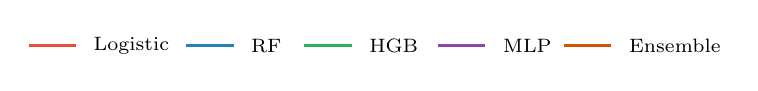
\begin{tikzpicture}
  \draw[thick, color=LogRegColor] (0,0) -- (0.6,0);
  \node[anchor=west, font=\scriptsize] at (0.7,0) {Logistic};
  \draw[thick, color=RFColor] (2.0,0) -- (2.6,0);
  \node[anchor=west, font=\scriptsize] at (2.7,0) {RF};
  \draw[thick, color=HGBColor] (3.5,0) -- (4.1,0);
  \node[anchor=west, font=\scriptsize] at (4.2,0) {HGB};
  \draw[thick, color=MLPColor] (5.2,0) -- (5.8,0);
  \node[anchor=west, font=\scriptsize] at (5.9,0) {MLP};
  \draw[thick, color=EnsColor] (6.8,0) -- (7.4,0);
  \node[anchor=west, font=\scriptsize] at (7.5,0) {Ensemble};
\end{tikzpicture}
\caption{ROC curves collapse near the upper-left corner on UCI, while Tawam preserves more visible separation.}
\end{figure}

\subsection{Power-Law Summaries}
\begin{figure}[H]
\centering
\begin{tikzpicture}
\begin{groupplot}[
  group style={group size=1 by 3, vertical sep=1.55cm},
  width=0.88\textwidth,
  height=0.28\textwidth,
  grid=major,
  grid style={draw=gray!20},
  xmode=log,
  ymin=0.55,
  ymax=1.02,
  tick align=inside,
  tick pos=left,
  tick label style={font=\small},
  label style={font=\small},
  title style={font=\bfseries\small},
]
\nextgroupplot[title={All features}, ylabel={HGB AUC}]
\addplot+[only marks, mark=o, color=HGBColor, forget plot] table[x=train_size,y=observed_hgb] {\DataDir/fig8_powerlaw_all.csv};
\addplot+[mark=none, thick, dashed, color=UCIRed, forget plot] table[x=train_size,y=fit_hgb] {\DataDir/fig8_powerlaw_all.csv};
\nextgroupplot[title={No eGFR/ACR}, ylabel={HGB AUC}]
\addplot+[only marks, mark=o, color=HGBColor, forget plot] table[x=train_size,y=observed_hgb] {\DataDir/fig8_powerlaw_no_egfr_acr.csv};
\addplot+[mark=none, thick, dashed, color=UCIRed, forget plot] table[x=train_size,y=fit_hgb] {\DataDir/fig8_powerlaw_no_egfr_acr.csv};
\nextgroupplot[title={No eGFR/ACR/Cr/BUN}, xlabel={Training size}, ylabel={HGB AUC}]
\addplot+[only marks, mark=o, color=HGBColor, forget plot] table[x=train_size,y=observed_hgb] {\DataDir/fig8_powerlaw_no_lab_surrogates.csv};
\addplot+[mark=none, thick, dashed, color=UCIRed, forget plot] table[x=train_size,y=fit_hgb] {\DataDir/fig8_powerlaw_no_lab_surrogates.csv};
\end{groupplot}
\end{tikzpicture}

\vspace{0.5em}
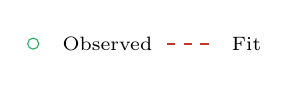
\begin{tikzpicture}
  \draw[only marks, mark=o, color=HGBColor] plot coordinates {(0,0)};
  \node[anchor=west, font=\scriptsize] at (0.25,0) {Observed};
  \draw[thick, dashed, color=UCIRed] (1.7,0) -- (2.3,0);
  \node[anchor=west, font=\scriptsize] at (2.4,0) {Fit};
\end{tikzpicture}
\caption{Power-law fits summarize NHANES learning behavior under the three feature definitions. The ceiling parameter is descriptive and constrained by AUC's upper bound.}
\end{figure}

\begin{table}[H]
\centering
\caption{NHANES power-law fit summaries. Values for $c$, $a$, and $b$ are estimate (95\% bootstrap CI). Drop--2 $c$ is the ceiling refit after excluding the two smallest training sizes.}
\scriptsize
\renewcommand{\arraystretch}{1.16}
\setlength{\tabcolsep}{2pt}
\begin{tabularx}{\textwidth}{|>{\raggedright\arraybackslash}p{1.25cm}|>{\centering\arraybackslash}X|>{\centering\arraybackslash}X|>{\centering\arraybackslash}X|>{\centering\arraybackslash}p{0.65cm}|>{\centering\arraybackslash}p{1.05cm}|}
\hline
\textbf{Model} & \textbf{$c$ ceiling} & \textbf{$a$} & \textbf{$b$} & \textbf{$R^2$} & \textbf{Drop--2 $c$} \\
\hline
\multicolumn{6}{|l|}{\textbf{All features}} \\
\hline
LogReg & 0.946 (0.946--0.953) & 1.736 (0.349--3.156) & 0.780 (0.427--0.929) & 0.990 & 0.950 \\
\hline
RF & 1.000 (1.000--1.000) & 1.446 (0.889--199.994) & 0.864 (0.746--1.774) & 0.980 & 1.000 \\
\hline
HGB & 1.000 (1.000--1.000) & 200.000 (14.296--200.000) & 1.637 (1.560--1.965) & 0.923 & 1.000 \\
\hline
MLP & 1.000 (1.000--1.000) & 4.790 (2.996--49.663) & 0.629 (0.513--1.053) & 0.948 & 1.000 \\
\hline
Ensemble & 1.000 (1.000--1.000) & 49.917 (45.269--199.971) & 1.668 (1.646--1.969) & 1.000 & 1.000 \\
\hline
\multicolumn{6}{|l|}{\textbf{No eGFR/ACR}} \\
\hline
LogReg & 0.813 (0.813--0.814) & 12.850 (1.612--22.715) & 1.305 (0.869--1.449) & 0.996 & 0.813 \\
\hline
RF & 0.974 (0.974--0.978) & 1.195 (0.402--1.461) & 0.731 (0.502--0.782) & 0.998 & 0.977 \\
\hline
HGB & 0.975 (0.975--0.989) & 200.000 (0.383--200.000) & 1.636 (0.428--1.642) & 0.972 & 0.981 \\
\hline
MLP & 1.000 (0.972--1.000) & 2.658 (1.571--200.000) & 0.448 (0.318--1.211) & 0.859 & 0.973 \\
\hline
Ensemble & 0.975 (0.975--0.986) & 3.498 (0.172--9.804) & 0.946 (0.303--1.203) & 0.978 & 0.985 \\
\hline
\multicolumn{6}{|l|}{\textbf{No eGFR/ACR/Cr/BUN}} \\
\hline
LogReg & 0.693 (0.693--0.696) & 4.643 (0.772--9.046) & 1.038 (0.655--1.204) & 0.995 & 0.694 \\
\hline
RF & 0.922 (0.921--0.925) & 2.417 (0.910--2.573) & 0.786 (0.589--0.803) & 0.999 & 0.925 \\
\hline
HGB & 0.919 (0.919--0.953) & 200.000 (0.228--200.000) & 1.672 (0.201--1.680) & 0.973 & 0.947 \\
\hline
MLP & 1.000 (0.918--1.000) & 1.782 (1.284--129.410) & 0.325 (0.246--1.113) & 0.869 & 0.921 \\
\hline
Ensemble & 0.921 (0.921--0.938) & 5.530 (0.217--17.151) & 0.968 (0.276--1.251) & 0.975 & 0.937 \\
\hline
\end{tabularx}
\end{table}

\section{Discussion}
\subsection{The UCI Ceiling}
Three lines of evidence support the interpretation that UCI is not a useful general benchmark for CKD machine learning progress. First, many common models achieve nearly identical near-perfect performance. Second, learning curves saturate after very small training sizes. Third, several individual variables are already highly discriminative. Together, these results suggest that UCI primarily measures recognition of late-stage CKD in a hospital-like case-control setting, a concern that fits broader warnings about small benchmark datasets and overoptimistic model validation \cite{vabalas2019,collins2024}.

\subsection{Right Problem, Wrong Population}
The issue is not that UCI is useless. It answers a narrow question: can models separate advanced CKD cases from healthy controls in a hospital-derived dataset? The clinically urgent early-screening question is different. UCI can remain useful for teaching, debugging, and demonstrating preprocessing pipelines, but strong UCI performance should not be treated as evidence of real-world CKD screening utility without external validation \cite{collins2024,zech2018}.

\subsection{NHANES Circularity}
NHANES demonstrates a related but distinct problem. When eGFR and ACR are included as predictors, the label is partly contained inside the feature set because CKD classification is organized around kidney filtration and albuminuria criteria \cite{kdigo2024}. Removing these variables, and then removing creatinine and BUN surrogates, lowers performance in a monotonic pattern. This shows that ceiling effects can come from either extreme disease separation or label-feature overlap.

\subsection{Ablation Interpretation}
The UCI ablation result is more nuanced than a simple shortcut story. The top three single features are highly discriminative, but removing them does not materially reduce performance. This suggests that the UCI ceiling is redundant across multiple late-stage biomarker abnormalities rather than driven by one fragile leaking variable, which is consistent with the broader shortcut-learning idea that models can exploit several correlated cues rather than one explicit leakage variable \cite{geirhos2020,ongly2024}.

\subsection{Implications}
The broader implication is methodological. AUC values near 1.0 on small single-cohort CKD datasets should not automatically be interpreted as model superiority. External validation, learning curves, single-feature screening, feature-set sensitivity analysis, and calibration or threshold checks should be routine parts of CKD model reporting \cite{vabalas2019,collins2024,ongly2024,hill2024}. The calibration and threshold results show why discrimination alone can mislead: on Tawam, random forest and the ensemble have high AUCs but threshold 0.5 sensitivities of only 0.143 and 0.286, respectively, meaning that default thresholds would miss many future CKD cases. The practical recommendations in this paper are hypotheses from one CKD case study, not universal rules.

\subsection{Limitations}
This study relies on public secondary datasets and inherits their cohort and measurement limitations. Tawam is a single-center cohort with only 56 events, so its overfitting checks should be interpreted as a warning about stability rather than as a definitive external validation study \cite{alshamsi2018,vabalas2019}. NHANES is analyzed as an ML benchmark rather than a weighted population survey, so no population-prevalence claims are made and the results should not be read as nationally representative estimates \cite{nhanes2024brief}. Cross-dataset transfer is conservative because only a small shared feature subset can be used. Power-law ceilings are model- and feature-set-dependent extrapolations rather than biological limits, especially when fitted parameters hit upper bounds. The analysis does not audit demographic fairness or subgroup calibration, which are important concerns for clinical machine learning \cite{yang2023}, and it does not include newer tabular foundation models such as TabPFN \cite{hollmann2025}.

\subsection{Concluding Remarks}
UCI should not be discarded entirely, but it should stop being treated as a general benchmark for progress in CKD machine learning. It remains useful for teaching tasks such as demonstrating train/test splits, missing-value imputation, categorical encoding, and basic model comparison. The revised analysis shows that realistic CKD prediction tasks produce lower AUCs, slower learning curves, and more meaningful algorithmic differences, while UCI remains saturated even after top-feature ablation and transfers poorly to external CKD settings. The transfer result should be read conservatively because only three shared predictors could be aligned across datasets.

\subsection{Data and Code Availability}
The analysis code is included with this manuscript as \texttt{nhsjs.py} and is available in the \href{https://github.com/jxia2027-cloud/NHSJS.git}{GitHub repository}. Regenerated outputs are included as \texttt{outputs/results.json} and as CSV files in \texttt{outputs/latex\_data/}. These files contain only de-identified derived data tables and model-output summaries used to render the LaTeX figures and tables.

\section{Acknowledgments}
The author thanks the UCI Machine Learning Repository, CDC/NCHS for NHANES 2021--2023, Tawam Hospital for the published CKD cohort, and American Heritage School for supporting independent research.

\begin{thebibliography}{26}
\bibitem{bikbov2020} B. Bikbov, C. A. Purcell, A. S. Levey, et al. Global, regional, and national burden of chronic kidney disease, 1990--2017: a systematic analysis for the Global Burden of Disease Study 2017. \emph{Lancet.} Vol. 395, No. 10225, pg. 709--733, 2020, DOI: \url{https://doi.org/10.1016/S0140-6736(20)30045-3}.
\bibitem{levey2012} A. S. Levey and J. Coresh. Chronic kidney disease. \emph{Lancet.} Vol. 379, No. 9811, pg. 165--180, 2012, DOI: \url{https://doi.org/10.1016/S0140-6736(11)60178-5}.
\bibitem{rubini2015} L. J. Rubini, P. Soundarapandian, and P. Eswaran. Chronic kidney disease. UCI Machine Learning Repository, 2015, DOI: \url{https://doi.org/10.24432/C5G020}.
\bibitem{salekin2016} A. Salekin and J. Stankovic. Detection of chronic kidney disease and selecting important predictive attributes. \emph{2016 IEEE International Conference on Healthcare Informatics (ICHI).} pg. 262--270, 2016, DOI: \url{https://doi.org/10.1109/ICHI.2016.36}.
\bibitem{islam2023} M. A. Islam, M. Z. H. Majumder, and M. A. Hussein. Chronic kidney disease prediction based on machine learning algorithms. \emph{Journal of Pathology Informatics.} Vol. 14, article 100189, 2023, DOI: \url{https://doi.org/10.1016/j.jpi.2023.100189}.
\bibitem{chittora2021} P. Chittora, S. Chaurasia, P. Chakrabarti, et al. Prediction of chronic kidney disease: a machine learning perspective. \emph{IEEE Access.} Vol. 9, pg. 17312--17334, 2021, DOI: \url{https://doi.org/10.1109/ACCESS.2021.3053763}.
\bibitem{kdigo2024} KDIGO CKD Work Group. KDIGO 2024 clinical practice guideline for the evaluation and management of chronic kidney disease. \emph{Kidney International.} Vol. 105, No. 4S, pg. S117--S314, 2024, DOI: \url{https://doi.org/10.1016/j.kint.2023.10.018}.
\bibitem{zech2018} J. R. Zech, M. A. Badgeley, M. Liu, et al. Variable generalization performance of a deep learning model to detect pneumonia in chest radiographs: a cross-sectional study. \emph{PLOS Medicine.} Vol. 15, No. 11, article e1002683, 2018, DOI: \url{https://doi.org/10.1371/journal.pmed.1002683}.
\bibitem{geirhos2020} R. Geirhos, J. H. Jacobsen, C. Michaelis, et al. Shortcut learning in deep neural networks. \emph{Nature Machine Intelligence.} Vol. 2, pg. 665--673, 2020, DOI: \url{https://doi.org/10.1038/s42256-020-00257-z}.
\bibitem{cdc2024} Centers for Disease Control and Prevention, National Center for Health Statistics. NHANES August 2021--August 2023 questionnaires, datasets, and related documentation. 2024, URL: \url{https://wwwn.cdc.gov/nchs/nhanes/continuousnhanes/default.aspx?Cycle=2021-2023}.
\bibitem{nhanes2024brief} Centers for Disease Control and Prevention, National Center for Health Statistics. Brief overview of sample design, nonresponse bias assessment, and analytic guidelines for NHANES August 2021--August 2023. 2024, URL: \url{https://wwwn.cdc.gov/nchs/NHANES/continuousnhanes/overviewbrief.aspx?cycle=2021-2023}.
\bibitem{alshamsi2018} S. Al-Shamsi, D. Regmi, and R. D. Govender. Chronic kidney disease in patients at high risk of cardiovascular disease in the United Arab Emirates: a population-based study. \emph{PLOS ONE.} Vol. 13, No. 6, article e0199920, 2018, DOI: \url{https://doi.org/10.1371/journal.pone.0199920}.
\bibitem{hollmann2025} N. Hollmann, S. Muller, L. Purucker, et al. Accurate predictions on small data with a tabular foundation model. \emph{Nature.} Vol. 637, pg. 319--326, 2025, DOI: \url{https://doi.org/10.1038/s41586-024-08328-6}.
\bibitem{ganie2023} S. M. Ganie, P. K. Dutta Pramanik, S. Mallik, and Z. Zhao. Chronic kidney disease prediction using boosting techniques based on clinical parameters. \emph{PLOS ONE.} Vol. 18, No. 12, article e0295234, 2023, DOI: \url{https://doi.org/10.1371/journal.pone.0295234}.
\bibitem{halder2024} R. K. Halder, M. N. Uddin, M. A. Uddin, et al. ML-CKDP: machine learning-based chronic kidney disease prediction with smart web application. \emph{Journal of Pathology Informatics.} Vol. 15, article 100371, 2024, DOI: \url{https://doi.org/10.1016/j.jpi.2024.100371}.
\bibitem{dritsas2022} E. Dritsas and M. Trigka. Machine learning techniques for chronic kidney disease risk prediction. \emph{Big Data and Cognitive Computing.} Vol. 6, No. 3, article 98, 2022, DOI: \url{https://doi.org/10.3390/bdcc6030098}.
\bibitem{chen2025} H. Chen, Y. Huang, and L. Chen. Ensemble machine learning for predicting renal function decline in chronic kidney disease: development and external validation. \emph{Frontiers in Medicine.} Vol. 12, article 1598065, 2025, DOI: \url{https://doi.org/10.3389/fmed.2025.1598065}.
\bibitem{collins2024} G. S. Collins, K. G. M. Moons, P. Dhiman, et al. TRIPOD+AI statement: updated guidance for reporting clinical prediction models that use regression or machine learning methods. \emph{BMJ.} Vol. 385, article e078378, 2024, DOI: \url{https://doi.org/10.1136/bmj-2023-078378}.
\bibitem{ongly2024} C. Ong Ly, B. Unnikrishnan, T. Tadic, et al. Shortcut learning in medical AI hinders generalization: method for estimating AI model generalization without external data. \emph{npj Digital Medicine.} Vol. 7, article 124, 2024, DOI: \url{https://doi.org/10.1038/s41746-024-01118-4}.
\bibitem{hill2024} B. G. Hill, F. L. Koback, and P. L. Schilling. The risk of shortcutting in deep learning algorithms for medical imaging research. \emph{Scientific Reports.} Vol. 14, article 29224, 2024, DOI: \url{https://doi.org/10.1038/s41598-024-79838-6}.
\bibitem{dayimu2024} A. Dayimu, N. Simidjievski, N. Demiris, and J. Abraham. Sample size determination for prediction models via learning-type curves. \emph{Statistics in Medicine.} Vol. 43, No. 16, pg. 3062--3072, 2024, DOI: \url{https://doi.org/10.1002/sim.10121}.
\bibitem{vabalas2019} A. Vabalas, E. Gowen, E. Poliakoff, and A. J. Casson. Machine learning algorithm validation with a limited sample size. \emph{PLOS ONE.} Vol. 14, No. 11, article e0224365, 2019, DOI: \url{https://doi.org/10.1371/journal.pone.0224365}.
\bibitem{meek2002} C. Meek, B. Thiesson, and D. Heckerman. The learning-curve sampling method applied to model-based clustering. \emph{Journal of Machine Learning Research.} Vol. 2, pg. 397--418, 2002.
\bibitem{yang2023} J. Yang, A. A. S. Soltan, D. W. Eyre, and D. A. Clifton. Algorithmic fairness and bias mitigation for clinical machine learning with deep reinforcement learning. \emph{Nature Machine Intelligence.} Vol. 5, No. 8, pg. 884--894, 2023, DOI: \url{https://doi.org/10.1038/s42256-023-00697-3}.
\bibitem{li2025} J. Li, X. Du, R. Zhang, et al. Machine learning models for predicting short-term progression in patients with stage 4 chronic kidney disease: a multi-center validation study. \emph{Scientific Reports.} Vol. 15, article 39285, 2025, DOI: \url{https://doi.org/10.1038/s41598-025-23037-4}.
\bibitem{shu2026} P. Shu, D. Qin, F. Xu, L. Guo, Z. Wen, and X. Wang. Development and internal validation of an interpretable machine learning model for predicting dialysis risk in patients with stage 3--4 chronic kidney disease. \emph{Frontiers in Public Health.} Vol. 14, article 1782951, 2026, DOI: \url{https://doi.org/10.3389/fpubh.2026.1782951}.
\end{thebibliography}

\end{document}
